\chapter{Frequency sweep matching}
\section{Outline of the system}
Computer 1 will set the capacitors $C_p$,$C_s$ and $C_a$ on capacitances
\begin{eqnarray}
	a &\in (\text{35pF},\text{1000pF})\\
	s &\in (\text{25pF},\text{1000pF})\\
	p &\in (\text{7pF},\text{1000pF})
\end{eqnarray}
And start a \textit{Frequency sweep} i.e vary the frequency over some interval
(relevant to ICRH, e.g 10-55MHz), keeping the power constant.\\ The waveguide
is equipped with a differential coupler, making it possible to measure the
amplitude of the reflected signal. This way we can see it make a dip at the
"matched" frequency, let's for now quantify the discrepency between the
required/requested frequency $f_r$ and the matched frequency $f_m$ using
\begin{equation}
	\Delta f^2 = f_m^2 - f_r^2
\end{equation}
Our goal is thus to minimize $\Delta f$ (note that we throw some information
away by making it positive definite, this won't become a problem as will be shown),
making the matched frequency corresponding to the system as close as possible
to the frequency we want. To do this we'll send the frequency sweep data over
from computer 2 (DAQ) to computer 1 (GUI), find $f_m$ by seeking the minimum of
the reflected signal, compute $\Delta f$, feed this into a program which
manipulates the capacitors to try and bring this value to zero, and repeat.
This system is shown in figure 
\ref{fig:system}.
\begin{figure}[h]
	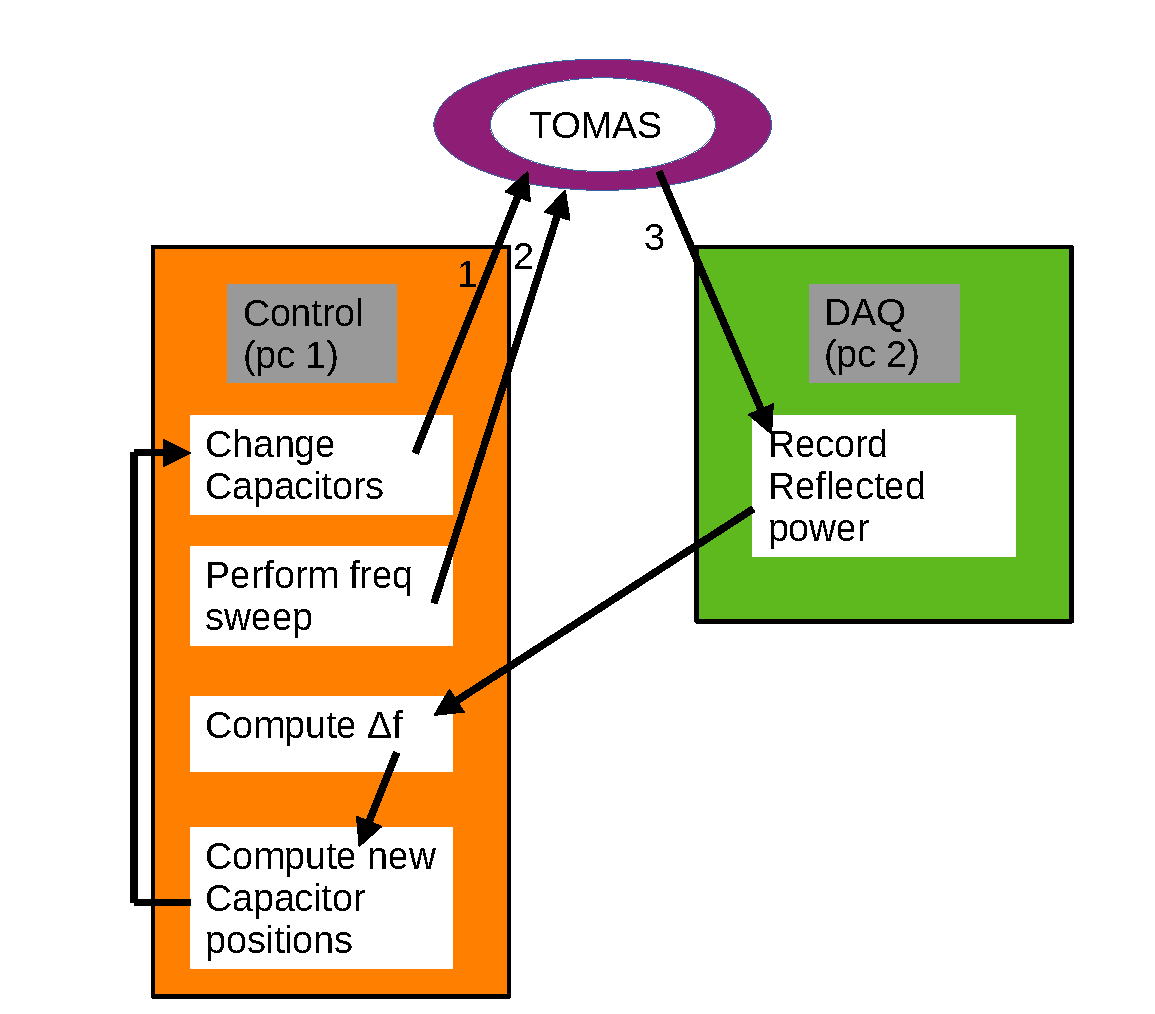
\includegraphics[width=\textwidth]{System.pdf}
	\caption{Overview of the system, pc2 will communicate with pc1 through TCP/IP}
	\label{fig:system}
\end{figure}
\section{Algorithm}
It's all well and good to think out a way to change everything in steps but the biggest problem
is still the same: how should the capacitances be chosen i.f.o $\Delta f$?
I.e what does the 3-dimensional function
\begin{equation}
	\vec{f}(\Delta f) = \vec{C} = \begin{bmatrix}
a\\
p\\
s\\
\end{bmatrix}
\end{equation}
look like? Well let's start by eliminating the variable a as we'll just lower
it initially and heighten it after the matching is complete (hoping this
doesn't change the matched frequency too much). This leaves us with one input
for 2 outputs, we can however, using a a new power meter, also record the phase
of the reflected power $\Gamma_\phi$.  We can thus change the function to:
\begin{equation}
	\vec{f}(\Delta f, \Gamma_\phi) = 
	\begin{bmatrix}
	p\\
	s\\
	\end{bmatrix}
\end{equation}
Let's start by trying out a simple 
